% Gauss, Werke X/1 (1917), native leaves52–57, printed45–50.
\SourceLeaf{052}\ArithmeticHead{45}{R}{ÜBER GANZE KOMPLEXE ZAHLEN.}
\begin{center}Modulus $+5+8i,\quad D=89.$\end{center}
\begin{center}[\textit{Potenzen der Primitiv-Wurzel.}]\end{center}
\begin{ResidueTable}{r|r||r|r||r|r||r|r}
0&+1&6&-5&12&+4+2i&18&-2+i\\
1&+1-i&7&+3&13&-2+3i&19&-1+3i\\
2&-2i&8&+3-3i&14&-4-3i&20&+2+4i\\
3&-2-2i&9&+5+2i&15&+1-4i&21&+1-6i\\
4&-4&10&-1+2i&16&+2+3i&22&+i\\
5&+4-i&11&+1+3i&17&+5+i&&
\end{ResidueTable}
\IndexTitle
\begin{ResidueTable}{r|r||r|r||r|r||r|r}
+i&22&-3+2i&38&+1+6i&56&-7-2i&\\
+1+i&23&-3-2i&35&+1-6i&21&+5+6i&\\
+1-i&1&+1+4i&27&+5+4i&26&+5-6i&\\
+1+2i&84&+1-4i&15&+5-4i&33&-3+8i&\\
+1-2i&54&+5+2i&9&-7&83&-3-8i&\\
-3&51&+5-2i&52&-7+2i&63&+5-8i&
\end{ResidueTable}
\bigskip
\begin{center}Modulus $-3+8i,\quad D=73.$\end{center}
\PowerTitle
\begin{ResidueTable}{r|r||r|r||r|r||r|r}
0&+1&5&+4-i&10&+4-3i&15&-1-3i\\
1&+1+i&6&-3&11&-1-2i&16&-1+4i\\
2&+2i&7&-3-3i&12&+1-3i&17&-2-5i\\
3&-2+2i&8&-3+2i&13&+4-2i&18&+i\\
4&-4&9&+3+2i&14&-2-i&&
\end{ResidueTable}
\IndexTitle
\begin{ResidueTable}{r|r||r|r||r|r||r|r}
+i&18&-3+2i&8&+1+6i&13&-7-2i&1\\
+1+i&1&-3-2i&45&+1-6i&3&+5+6i&61\\
+1-i&55&+1+4i&23&+5+4i&69&+5-6i&57\\
+1+2i&47&+1-4i&52&+5-4i&31&-3-8i&62\\
+1-2i&32&+5+2i&66&-7&51&&\\
-3&6&+5-2i&35&-7+2i&10&&
\end{ResidueTable}
\clearpage

\SourceLeaf{053}\ArithmeticHead{46}{L}{ARITHMETIK.\quad NACHLASS.}
\begin{center}Modulus $+5+6i,\quad D=61.$\end{center}
\PowerTitle
\begin{ResidueTable}{r|r||r|r||r|r||r|r}
0&+1&4&-4&8&-1+4i&12&-3\\
1&-1-i&5&-1-2i&9&+1+2i&13&-2-3i\\
2&+2i&6&-1+3i&10&+3-i&14&+5\\
3&+2-2i&7&-2+3i&11&+1+4i&15&+i
\end{ResidueTable}
\IndexTitle
\begin{ResidueTable}{r|r||r|r||r|r||r|r}
+i&15&-3&12&+5+2i&19&+5-4i&46\\
+1+i&31&-3+2i&58&+5-2i&6&-7&53\\
+1-i&16&-3-2i&22&+1+6i&4&-7+2i&55\\
+1+2i&35&+1+4i&11&+1-6i&29&-7-2i&56\\
+1-2i&39&+1-4i&38&+5+4i&32&+5-6i&1
\end{ResidueTable}
\bigskip
\begin{center}Modulus $-7+2i,\quad D=53.$\end{center}
\PowerTitle
\begin{ResidueTable}{r|r||r|r||r|r||r|r}
0&+1&4&-4&8&-3i&12&-4-2i\\
1&+1+i&5&-2+3i&9&-4-i&13&+i\\
2&+2i&6&+2-i&10&+1+2i&&\\
3&-2+2i&7&+3+i&11&-3+i&&
\end{ResidueTable}
\IndexTitle
\begin{ResidueTable}{r|r||r|r||r|r||r|r}
+i&13&-3&47&+5+2i&51&+5-4i&16\\
+1+i&1&-3+2i&30&+5-2i&15&-7&28\\
+1-i&40&-3-2i&18&+1+6i&27&-7+2i&17\\
+1+2i&19&+1+4i&24&+1-6i&7&&\\
+1-2i&36&+1-4i&25&+5+4i&9&&
\end{ResidueTable}
\clearpage

\SourceLeaf{054}\ArithmeticHead{47}{R}{ÜBER GANZE KOMPLEXE ZAHLEN.}
\begin{center}Modulus $7,\quad D=49.$\end{center}
\PowerTitle
\begin{ResidueTable}{r|r||r|r||r|r||r|r}
0&+1&4&+3i&8&-2&12&+i\\
1&+1-2i&5&-1+3i&9&-2-3i&&\\
2&-3+3i&6&-2-2i&10&-1+i&&\\
3&+3+2i&7&+1+2i&11&+1+3i&&
\end{ResidueTable}
\IndexTitle
\begin{ResidueTable}{r|r||r|r||r|r||r|r}
+i&12&+1-2i&1&+1+4i&29&+1+6i&34\\
+1+i&46&-3&16&+1-4i&11&+1-6i&46\\
+1-i&34&-3+2i&45&+5+2i&42&+5+4i&9\\
+1+2i&7&-3-2i&27&+5-2i&6&+5-4i&15
\end{ResidueTable}
\bigskip
\begin{center}Modulus $+5+4i,\quad D=41.$\end{center}
\PowerTitle
\begin{ResidueTable}{r|r||r|r||r|r||r|r}
0&+1&3&+1-3i&6&+2+2i&9&-1-3i\\
1&-2+i&4&-2i&7&-1+2i&10&+i\\
2&-1+i&5&-3&8&-4&&
\end{ResidueTable}
\IndexTitle
\begin{ResidueTable}{r|r||r|r||r|r||r|r}
+i&10&+1-2i&27&+1+4i&8&+1+6i&15\\
+1+i&32&-3&5&+1-4i&39&+1-6i&33\\
+1-i&22&-3+2i&3&+5+2i&4&+5-4i&32\\
+1+2i&31&-3-2i&6&+5-2i&29&&
\end{ResidueTable}
\bigskip
\begin{center}Modulus $+1+6i,\quad D=37.$\end{center}
\PowerTitle
\begin{ResidueTable}{r|r||r|r||r|r||r|r}
0&+1&3&+2+2i&6&-1+2i&9&+i\\
1&-1+i&4&+2-i&7&-3i&&\\
2&-2i&5&-1+3i&8&-2+3i&&
\end{ResidueTable}
\clearpage

\SourceLeaf{055}\ArithmeticHead{48}{L}{ARITHMETIK.\quad NACHLASS.}
\IndexTitle
\begin{ResidueTable}{r|r||r|r||r|r||r|r}
+i&9&+1-2i&24&+1+4i&2&+1-6i&11\\
+1+i&28&-3&34&+1-4i&3&&\\
+1-i&19&-3+2i&32&+5+2i&5&&\\
+1+2i&13&-3-2i&17&+5-2i&10&&
\end{ResidueTable}
\begin{center}Modulus $+5+2i,\quad D=29.$\end{center}
\PowerTitle
\begin{ResidueTable}{r|r||r|r||r|r||r|r}
0&+1&2&-2i&4&+1+2i&6&-3+i\\
1&-1+i&3&+2+2i&5&+2+i&7&+i
\end{ResidueTable}
\IndexTitle
\begin{ResidueTable}{r|r||r|r||r|r||r|r}
+i&7&+1+2i&4&-3+2i&13&+1-4i&1\\
+1+i&22&+1-2i&26&-3-2i&9&+5-2i&11\\
+1-i&15&-3&3&+1+4i&20&&
\end{ResidueTable}
\begin{center}Modulus $+1+4i,\quad D=17.$\end{center}
\PowerTitle
\begin{ResidueTable}{r|r||r|r||r|r||r|r||r|r}
0&1&1&+1-2i&2&-2&3&+1-i&4&+i
\end{ResidueTable}
\IndexTitle
\begin{ResidueTable}{r|r||r|r||r|r||r|r||r|r}
+i&4&+1-i&3&+1-2i&1&-3+2i&7&+1-4i&10\\
+1+i&7&+1+2i&6&-3&3&-3-2i&5&&
\end{ResidueTable}
\begin{center}Modulus $-3+2i,\quad D=13.$\end{center}
\PowerTitle
\begin{ResidueTable}{r|r||r|r||r|r||r|r}
0&+1&1&+1-i&2&-2i&3&+i
\end{ResidueTable}
\IndexTitle
\begin{ResidueTable}{r|r||r|r||r|r||r|r}
+i&3&+1-i&1&+1-2i&11&-3-2i&7\\
+1+i&4&+1+2i&10&-3&2&&
\end{ResidueTable}
\clearpage

\SourceLeaf{056}\ArithmeticHead{49}{R}{ÜBER GANZE KOMPLEXE ZAHLEN.}
\begin{center}Modulus $3,\quad D=9.$\end{center}
\PowerTitle
\begin{ResidueTable}{r|r||r|r||r|r}
0&+1&1&+1-i&2&+i
\end{ResidueTable}
\IndexTitle
\begin{ResidueTable}{r|r||r|r||r|r||r|r}
+i&2&1+i&3&1+2i&1&1-2i&3
\end{ResidueTable}
\begin{center}Modulus $1+2i,\quad D=5.$\end{center}
\begin{center}\textit{Primitiv-Wurzel.}\end{center}
\[+i\]
\IndexTitle
\begin{ResidueTable}{r|r||r|r||r|r||r|r}
+i&1&1+i&3&1-i&2&1-2i&1
\end{ResidueTable}
\begin{center}
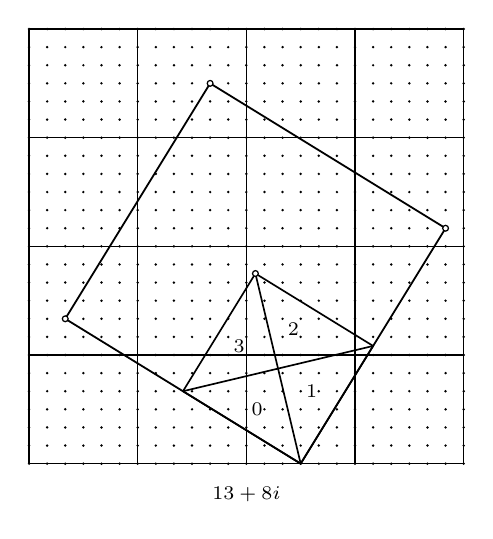
\begin{tikzpicture}[x=.23cm,y=.23cm,line width=.45pt,font=\scriptsize]
\foreach \x in {0,...,24}{\foreach \y in {0,...,24}{\fill (\x,\y) circle[radius=.075];}}
\foreach \x in {0,6,12,18,24}{\draw (\x,0)--(\x,24);}
\foreach \y in {0,6,12,18,24}{\draw (0,\y)--(24,\y);}
\draw[line width=.65pt] (2,8)--(10,21)--(23,13)--(15,0)--cycle;
\draw[line width=.6pt] (8.5,4)--(12.5,10.5)--(19,6.5)--(15,0)--cycle;
\draw[line width=.6pt] (12.5,10.5)--(15,0) (8.5,4)--(19,6.5);
\foreach \x/\y in {2/8,10/21,23/13,12.5/10.5}{\draw[fill=white] (\x,\y) circle[radius=.16];}
\node[fill=white,inner sep=.1pt] at (12.6,3.0) {$0$};
\node[fill=white,inner sep=.1pt] at (15.6,4.0) {$1$};
\node[fill=white,inner sep=.1pt] at (14.6,7.4) {$2$};
\node[fill=white,inner sep=.1pt] at (11.6,6.5) {$3$};
\node[below] at (12,-.7) {$13+8i$};
\end{tikzpicture}
\end{center}
\vfill\noindent\small X$_1$.\hfill7\par\normalsize
\clearpage

\SourceLeaf{057}\ArithmeticHead{50}{L}{ARITHMETIK.\quad NACHLASS.}
\begin{center}$481\quad\text{Div. per }9+20i$\end{center}
\begin{ResidueTable}{r|r}
52+169i&208+195i\\
65+91i&221+117i\\
78+13i&234+39i\\
130+182i&74+111i\\
143+104i&148+222i\\
156+26i&185+37i
\end{ResidueTable}
\bigskip
\begin{center}\textbf{BEMERKUNG.}\end{center}
\begingroup\small
\par\indent Zu der Notiz [2] vergleiche man die bezüglichen Bemerkungen im Artikel 21 des \textsc{Bachmann}schen Aufsatzes »Über \textsc{Gauss}' zahlentheoretische Arbeiten«.

Die Notiz [3] entspricht (nach einer Mitteilung von P. \textsc{Bachmann}) vollständig den bezüglichen Bestimmungen in der \textit{Commentatio secunda} (Werke II, S. 113 ff.) über biquadratische Reste. Die Tabellen geben für jeden der betrachteten Moduln zuerst die Reste\footnote{Es sind aber nicht überall die nach der im Text (S. 39) gegebenen Formel \textls[120]{kleinsten} Reste.} der ersten $\tfrac14(D-1)$ \textit{Potenzen einer primitiven Wurzel} bis zum Reste $i$, woraus die Reste der folgenden Potenzen leicht zu entnehmen sind. Dann folgen die \textit{Indizes} für die Einheit $i$ und die Primfaktoren $1+i$ und $\alpha+\beta i$, für die $\alpha\equiv1\ (\mathrm{mod.}\ 4)$ und die Norm $\alpha^2+\beta^2$ kleiner als $D$ ist, ausgenommen die Primzahl $a+bi$ selbst.

Für die Moduln $-3+2i$, $3$ und $1+2i$ steht in der Handschrift \textls[120]{Elementar-Wurzel} statt \textls[120]{Primitiv-Wurzel}.

Die Figur enthält in dem inneren, schief stehenden (in der Handschrift rot gezeichneten) großen Quadrat ein vollständiges Restsystem modulo $13+8i$, von dem durch das kleinere Quadrat ein Viertel abgetrennt ist.
\begin{flushright}\textsc{Schlesinger.}\end{flushright}
\ClosingRule\clearpage\endgroup
